\documentclass[11pt]{article}

\usepackage{latexsym}
\usepackage{amsmath}
\usepackage{amssymb}
\usepackage{amsthm}
\usepackage{graphicx}
\usepackage{wrapfig}
\usepackage{pseudocode}
\usepackage{url}
\usepackage[backref, colorlinks=true, citecolor=red, urlcolor=blue, pdfauthor={Jyh-Ming Lien}]{hyperref}
\usepackage{subfigure}

\newcommand{\handout}[5]{
  \noindent
  \begin{center}
  \framebox{
    \vbox{
      \hbox to 5.78in { {\bf } \hfill #2 }
      \vspace{4mm}
      \hbox to 5.78in { {\Large \hfill #5  \hfill} }
      \vspace{2mm}
      \hbox to 5.78in { {\em #3 \hfill #4} }
    }
  }
  \end{center}
  \vspace*{4mm}
}

\newcommand{\lecture}[4]{\handout{#1}{#2}{#3}{}{Report for #1}}

\newtheorem{theorem}{Theorem}
\newtheorem{corollary}[theorem]{Corollary}
\newtheorem{lemma}[theorem]{Lemma}
\newtheorem{observation}[theorem]{Observation}
\newtheorem{proposition}[theorem]{Proposition}
\newtheorem{definition}[theorem]{Definition}
\newtheorem{claim}[theorem]{Claim}
\newtheorem{fact}[theorem]{Fact}
\newtheorem{assumption}[theorem]{Assumption}

% 1-inch margins, from fullpage.sty by H.Partl, Version 2, Dec. 15, 1988.
\topmargin 0pt
\advance \topmargin by -\headheight
\advance \topmargin by -\headsep
\textheight 8.9in
\oddsidemargin 0pt
\evensidemargin \oddsidemargin
\marginparwidth 0.5in
\textwidth 6.5in

\parindent 0in
\parskip 1.5ex
%\renewcommand{\baselinestretch}{1.25}

\begin{document}

\lecture{Advance Algorithm Programming Assignment 1 }{Fall 2015}{Youngeun Lee}{---}


\section{Implementation Details}

The goal of this assignment is to compute Delaunay triangulation. I changed only Delaunay function in delanay.c. It has 3 steps as follow:
\begin{enumerate}
  \item Create points in 4D $(x,y,z,x^2+y^2+z^2)$
  \item Compute convex hull in 4D by qhull library\footnote{www.qhull.org/}
  \item Project the lower convex hull into 3D
\end{enumerate}
I will explain each steps in detail.

The first step is very easy. The vertices of the input file are stored in vertices. I made a pointer $(pt)$ of $coordT$ type and inserted the vertices and 4th coordinate.

The program calls qhull to compute convex hull in the second step. I referred to $QHull()$ function in main.c file. This function compute convex hull in 3D but the program should create convex hull in 4D. The option for qhull is $delaunay QJ Pp$. The pointer $pt$ is delivered to $qhull by qh_init_B()$ function. The 3th component of $qh\_init\_B()$ is 4 instead of 3 because I need to compute the convex hull in 4D.

The third step is difficult and I spent most of time in the step. The last coordinate of a normal from the convex hull determines that its tetrahedron is in upper side or lower side. The upper convex hull should look down the 4th axis. So the 4th normal value of the lower convex hull is less than zero. But it is not a enough condition for triangulation. A tetrahedron can be projected as a plane (Fig.~\ref{fig:coplanar}) since it lose one-dimension. These coplanar points occur crossed edges and faces. The program computes the volume of tetrahedron to avoid duplicated faces. $Volumei$ function in shape.c file computes a volume of a tetrahedron. The function returns 0 when the points of tetrahedron is coplanar. A tetrahedron which has 0 volume is not used to face construction.

\begin{figure}[!htb]
\centering
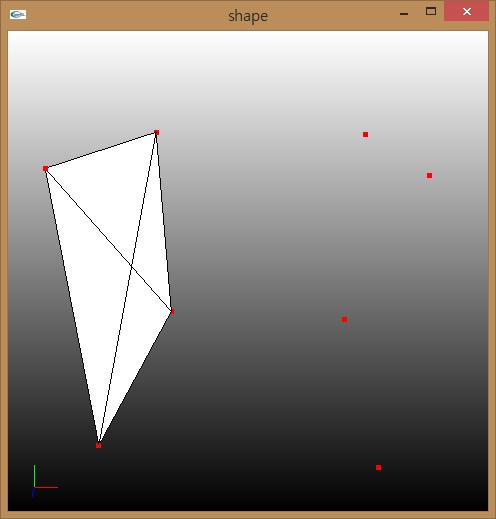
\includegraphics[height=5cm]{./figs/coplanar.jpg}
\caption{Coplanar Tetrahedron. The original model is $i.cube$. The 4 points are coplanar points, though they are components of a tetrahedron in 4D.}
\label{fig:coplanar}
\end{figure}  

I used Visual Studio 2012. I set up input argument $\%s$  $d ../../data/filename$ in the project property (Fig.~\ref{fig:input}).     

\begin{figure}[!htb]
\centering
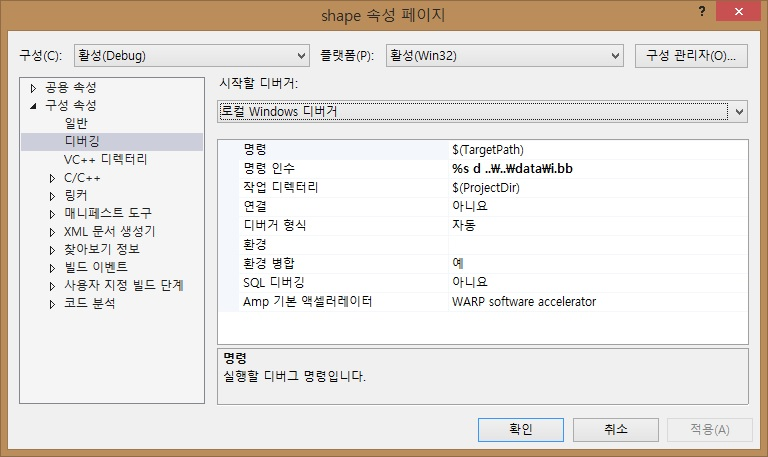
\includegraphics[height=7cm]{./figs/input.jpg}
\caption{Input argument.}
\label{fig:input}
\end{figure} 

\section{Example Output}

Fig.~\ref{fig:bb}, \ref{fig:bull}, \ref{fig:bunny}, \ref{fig:cube}, \ref{fig:ellipsoid}, \ref{fig:screwdriver}, \ref{fig:spoon}, \ref{fig:T}, \ref{fig:teeth}, \ref{fig:U}, \ref{fig:woman} and \ref{fig:Y} show results of each test file. The results of triangulation are not perfectly matching with given points because the program projects convex hulls. As you can see, there is no crossed faces and edges.

\begin{figure}[!htb]
\centering
\subfigure[Faces and vertices]{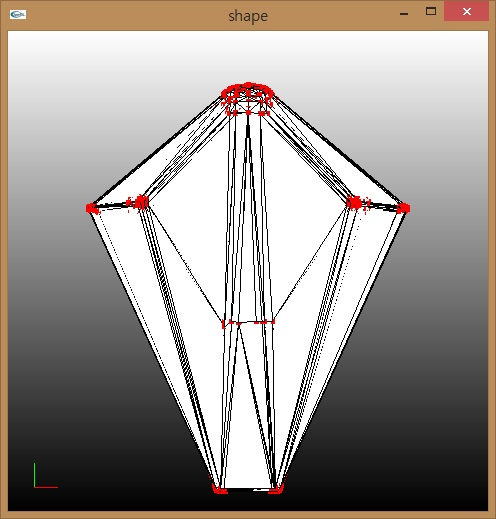
\includegraphics[height=4.0cm]{./figs/bb_f.jpg}}
\subfigure[Edges and vertices]{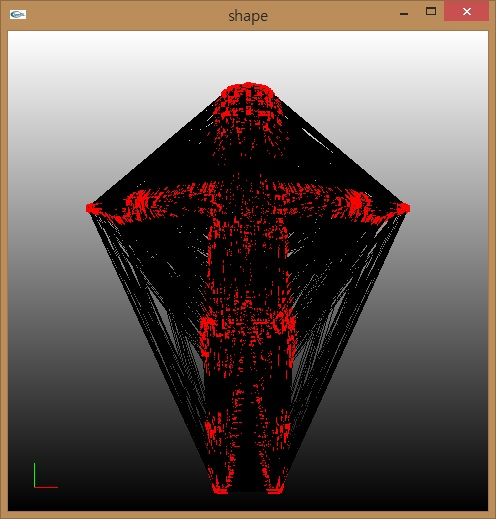
\includegraphics[height=4.0cm]{./figs/bb_e.jpg}}
\subfigure[Vertices]{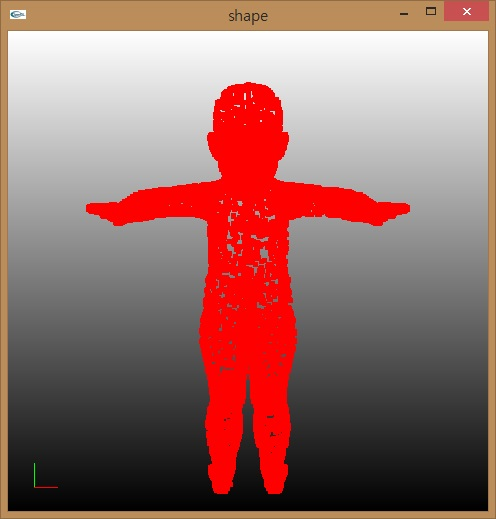
\includegraphics[height=4.0cm]{./figs/bb_v.jpg}}
\subfigure[Tetrahedrons]{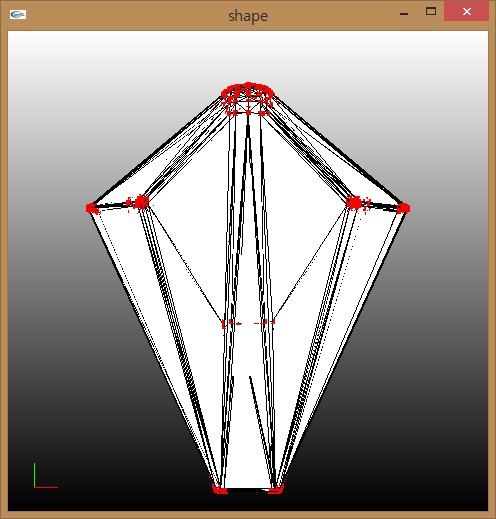
\includegraphics[height=4.0cm]{./figs/bb_t.jpg}}
\caption{i.bb}
\label{fig:bb}
\end{figure}

\begin{figure}[!htb]
\centering
\subfigure[Faces and vertices]{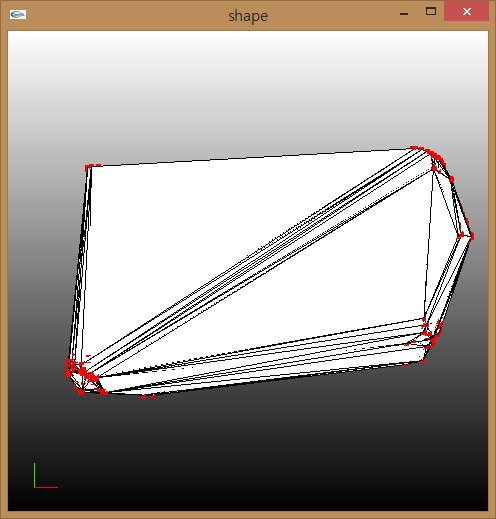
\includegraphics[height=4.0cm]{./figs/bull_f.jpg}}
\subfigure[Edges and vertices]{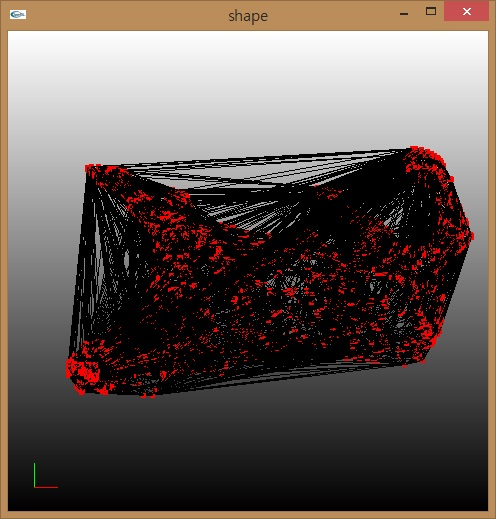
\includegraphics[height=4.0cm]{./figs/bull_e.jpg}}
\subfigure[Vertices]{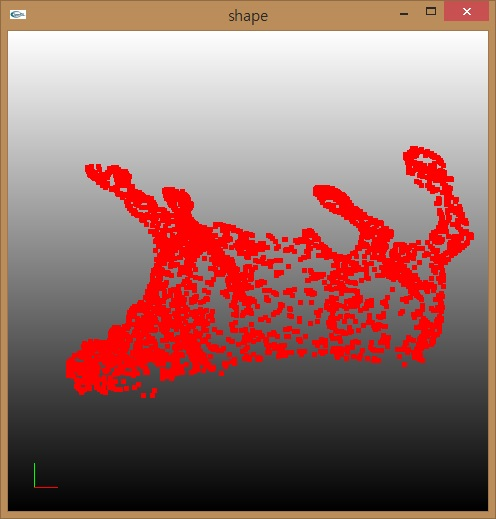
\includegraphics[height=4.0cm]{./figs/bull_v.jpg}}
\subfigure[Tetrahedrons]{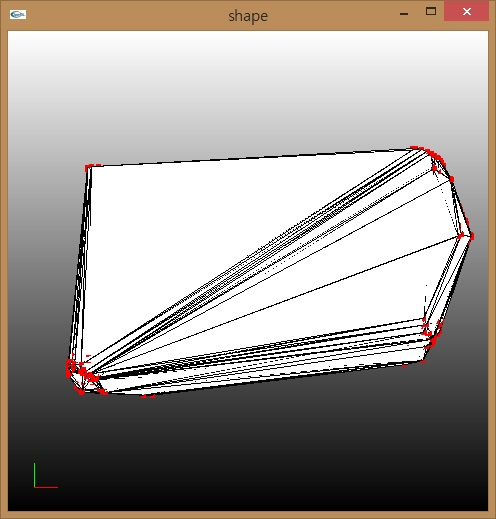
\includegraphics[height=4.0cm]{./figs/bull_t.jpg}}
\caption{i.bull}
\label{fig:bull}
\end{figure}

\begin{figure}[!htb]
\centering
\subfigure[Faces and vertices]{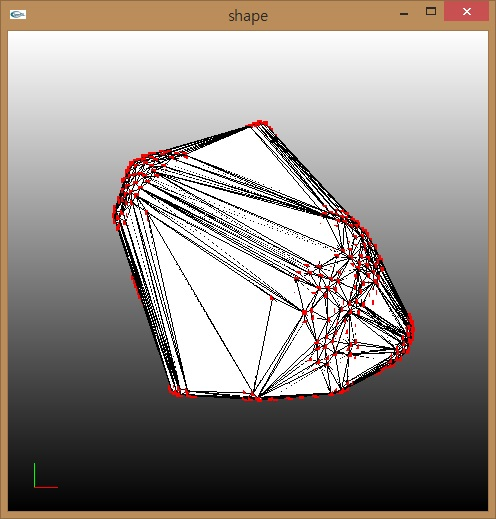
\includegraphics[height=4.0cm]{./figs/bunny_f.jpg}}
\subfigure[Edges and vertices]{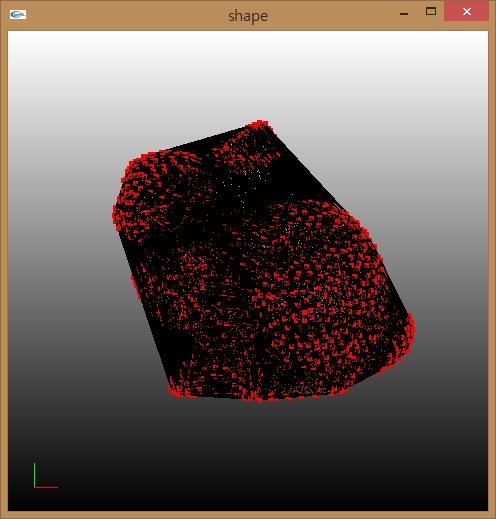
\includegraphics[height=4.0cm]{./figs/bunny_e.jpg}}
\subfigure[Vertices]{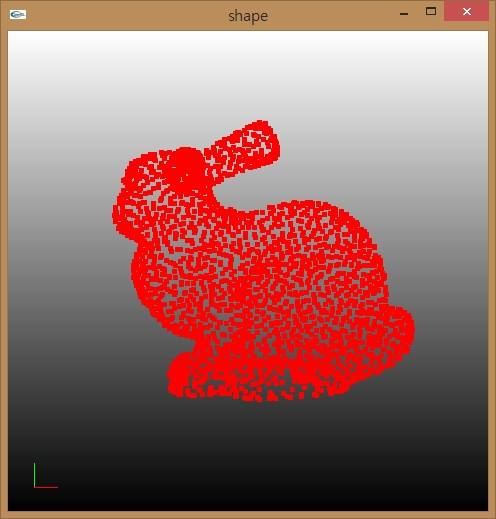
\includegraphics[height=4.0cm]{./figs/bunny_v.jpg}}
\subfigure[Tetrahedrons]{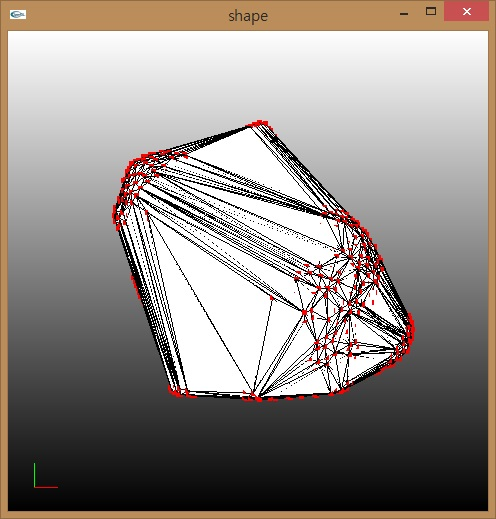
\includegraphics[height=4.0cm]{./figs/bunny_t.jpg}}
\caption{i.bunny}
\label{fig:bunny}
\end{figure}

\begin{figure}[!htb]
\centering
\subfigure[Faces and vertices]{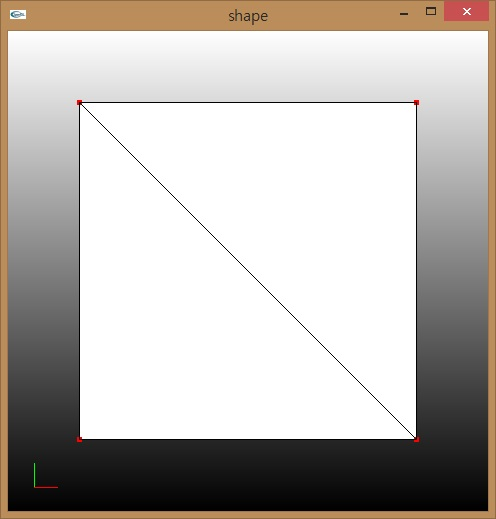
\includegraphics[height=4.0cm]{./figs/cube_f.jpg}}
\subfigure[Edges and vertices]{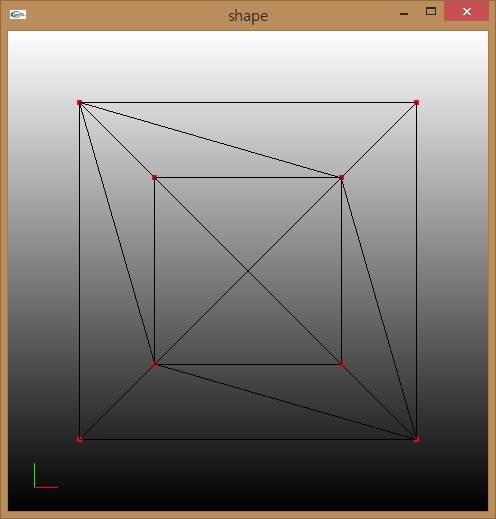
\includegraphics[height=4.0cm]{./figs/cube_e.jpg}}
\subfigure[Vertices]{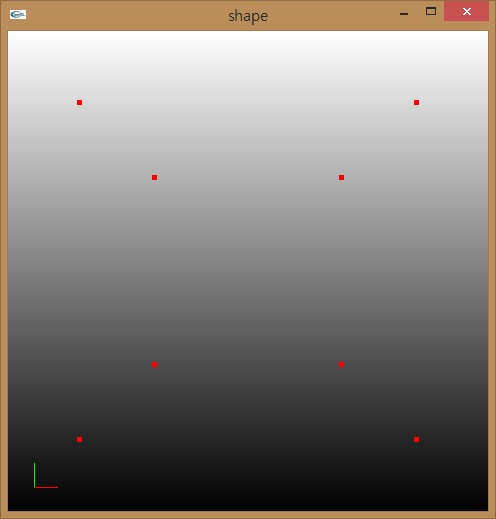
\includegraphics[height=4.0cm]{./figs/cube_v.jpg}}
\subfigure[Tetrahedrons]{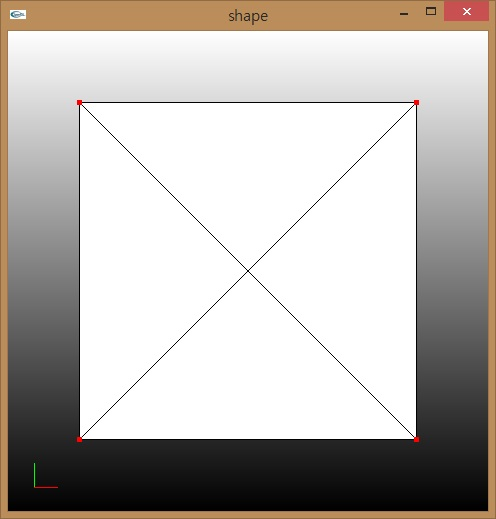
\includegraphics[height=4.0cm]{./figs/cube_t.jpg}}
\caption{i.cube}
\label{fig:cube}
\end{figure}

\begin{figure}[!htb]
\centering
\subfigure[Faces and vertices]{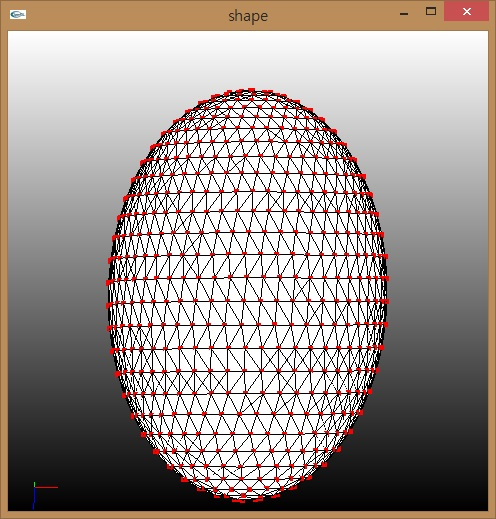
\includegraphics[height=4.0cm]{./figs/ellipsoid_f.jpg}}
\subfigure[Edges and vertices]{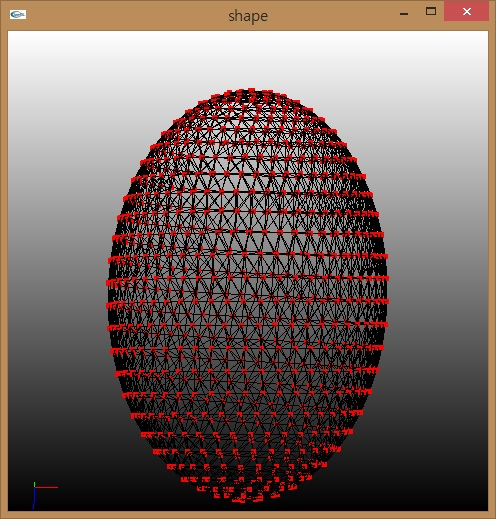
\includegraphics[height=4.0cm]{./figs/ellipsoid_e.jpg}}
\subfigure[Vertices]{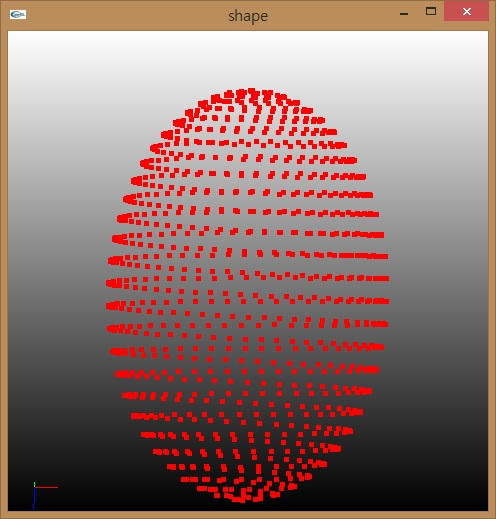
\includegraphics[height=4.0cm]{./figs/ellipsoid_v.jpg}}
\subfigure[Tetrahedrons]{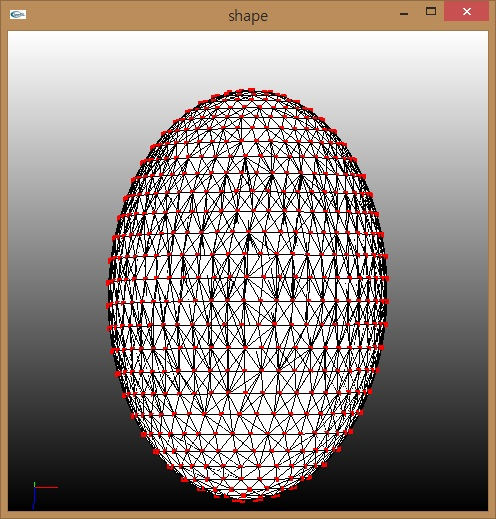
\includegraphics[height=4.0cm]{./figs/ellipsoid_t.jpg}}
\caption{i.ellipsoid}
\label{fig:ellipsoid}
\end{figure}

\begin{figure}[!htb]
\centering
\subfigure[Faces and vertices]{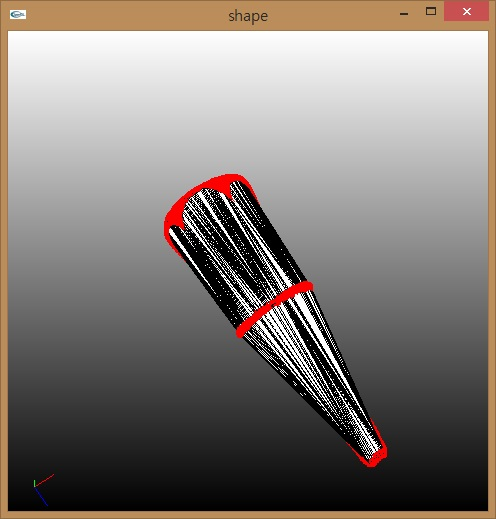
\includegraphics[height=4.0cm]{./figs/screwdriver_f.jpg}}
\subfigure[Edges and vertices]{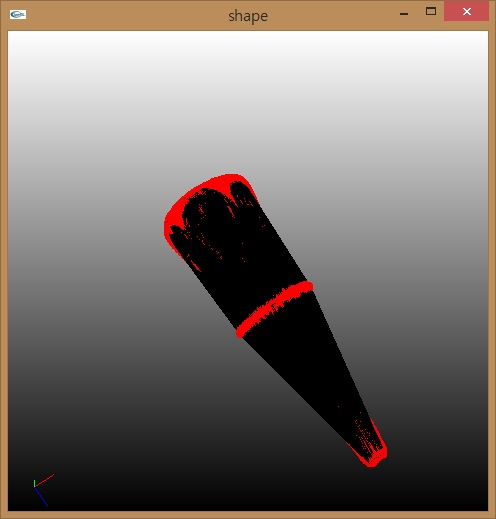
\includegraphics[height=4.0cm]{./figs/screwdriver_e.jpg}}
\subfigure[Vertices]{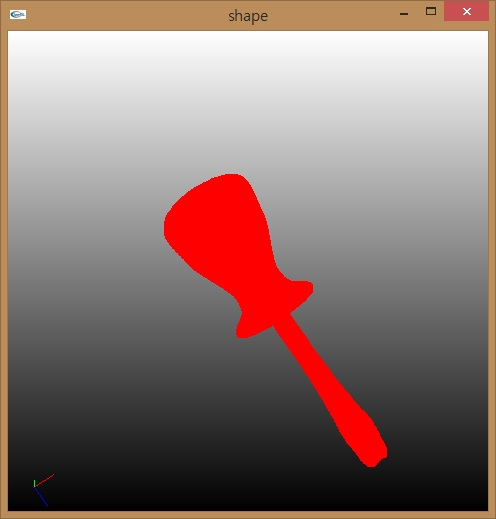
\includegraphics[height=4.0cm]{./figs/screwdriver_v.jpg}}
\subfigure[Tetrahedrons]{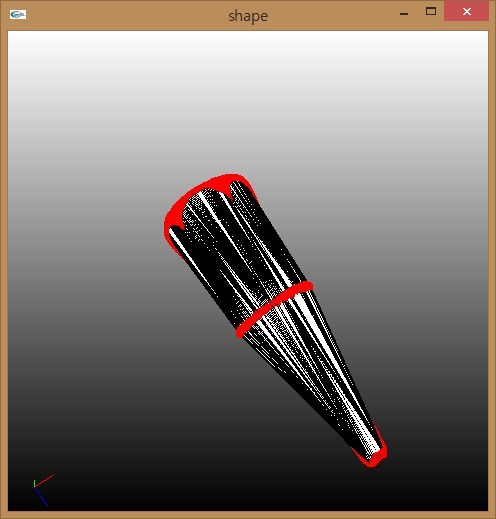
\includegraphics[height=4.0cm]{./figs/screwdriver_t.jpg}}
\caption{i.screwdriver}
\label{fig:screwdriver}
\end{figure}

\begin{figure}[!htb]
\centering
\subfigure[Faces and vertices]{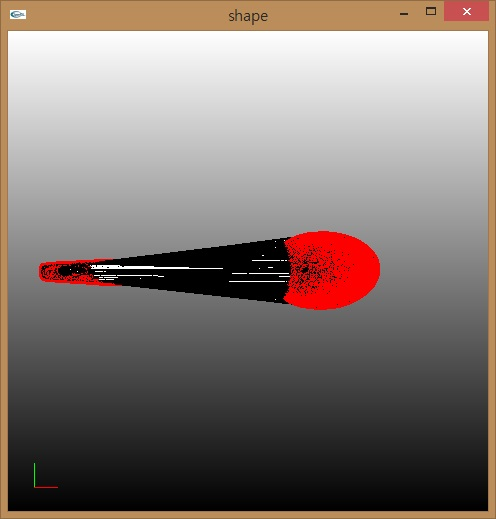
\includegraphics[height=4.0cm]{./figs/spoon_f.jpg}}
\subfigure[Edges and vertices]{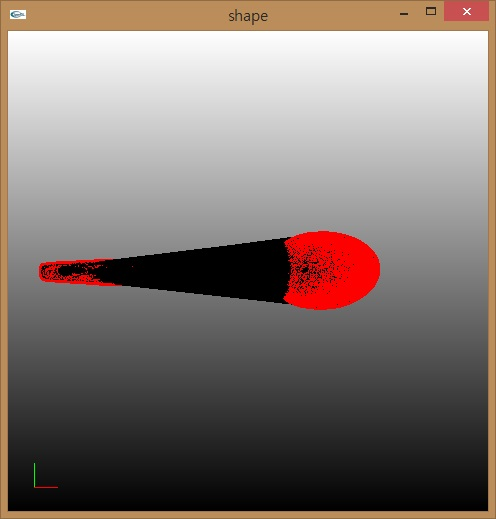
\includegraphics[height=4.0cm]{./figs/spoon_e.jpg}}
\subfigure[Vertices]{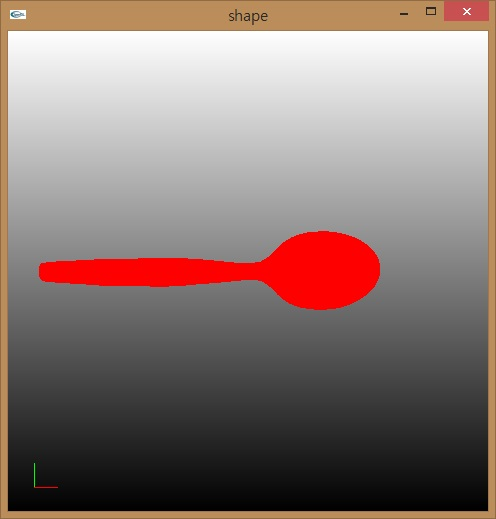
\includegraphics[height=4.0cm]{./figs/spoon_v.jpg}}
\subfigure[Tetrahedrons]{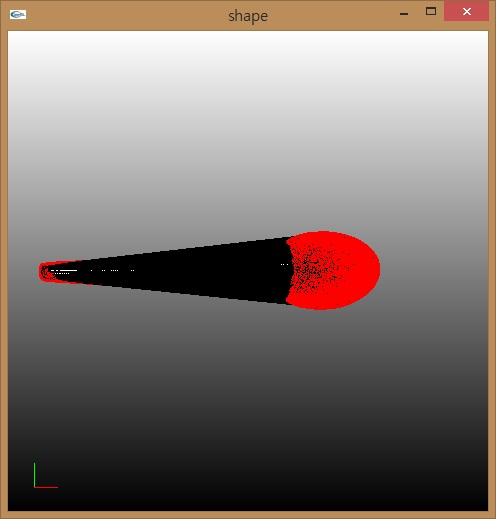
\includegraphics[height=4.0cm]{./figs/spoon_t.jpg}}
\caption{i.spoon}
\label{fig:spoon}
\end{figure}

\begin{figure}[!htb]
\centering
\subfigure[Faces and vertices]{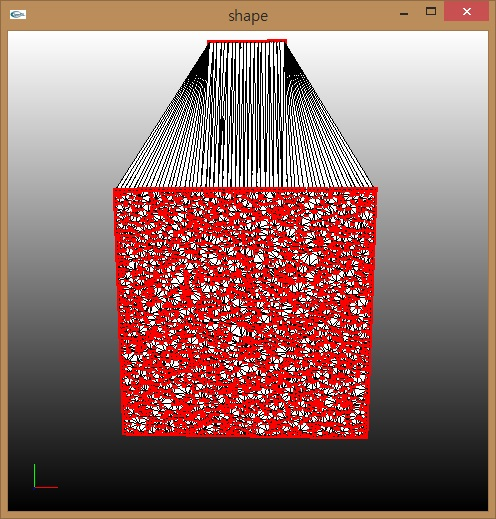
\includegraphics[height=4.0cm]{./figs/T_f.jpg}}
\subfigure[Edges and vertices]{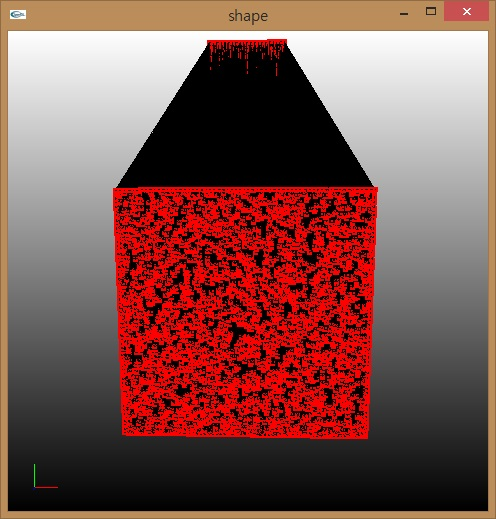
\includegraphics[height=4.0cm]{./figs/T_e.jpg}}
\subfigure[Vertices]{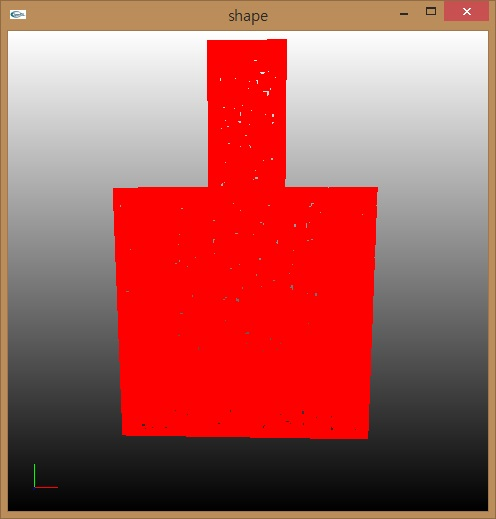
\includegraphics[height=4.0cm]{./figs/T_v.jpg}}
\subfigure[Tetrahedrons]{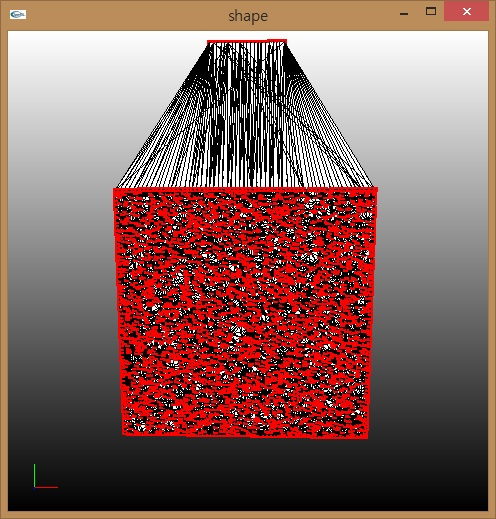
\includegraphics[height=4.0cm]{./figs/T_t.jpg}}
\caption{i.T}
\label{fig:T}
\end{figure}

\begin{figure}[!htb]
\centering
\subfigure[Faces and vertices]{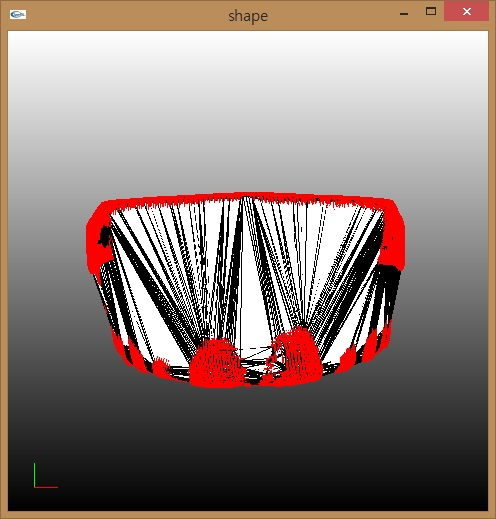
\includegraphics[height=4.0cm]{./figs/teeth_f.jpg}}
\subfigure[Edges and vertices]{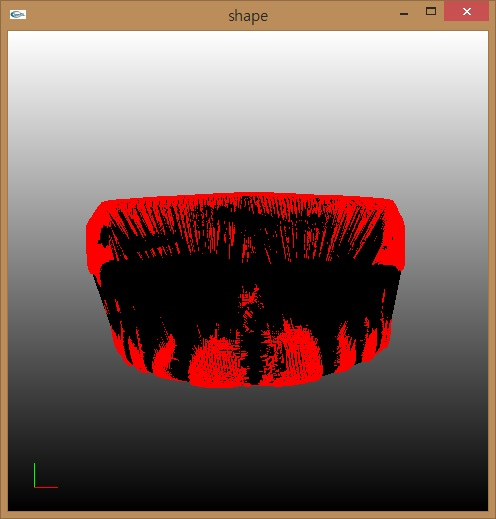
\includegraphics[height=4.0cm]{./figs/teeth_e.jpg}}
\subfigure[Vertices]{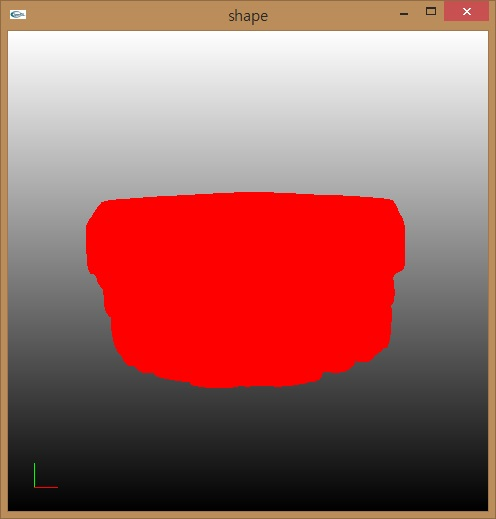
\includegraphics[height=4.0cm]{./figs/teeth_v.jpg}}
\subfigure[Tetrahedrons]{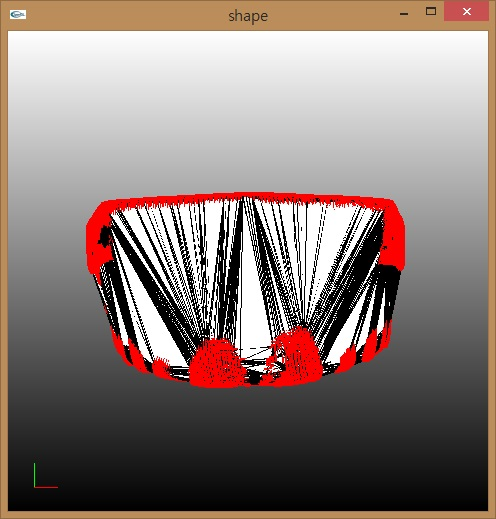
\includegraphics[height=4.0cm]{./figs/teeth_t.jpg}}
\caption{i.teeth}
\label{fig:teeth}
\end{figure}

\begin{figure}[!htb]
\centering
\subfigure[Faces and vertices]{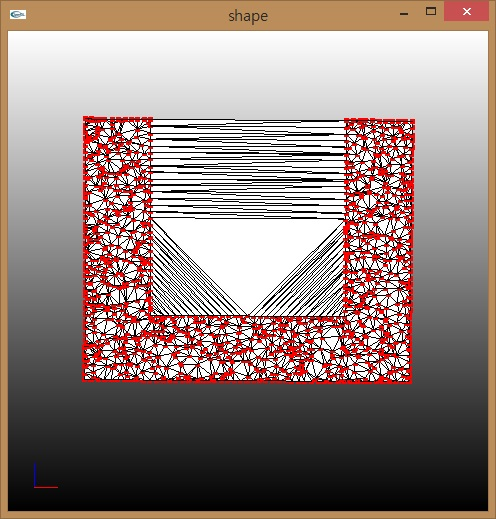
\includegraphics[height=4.0cm]{./figs/U_f.jpg}}
\subfigure[Edges and vertices]{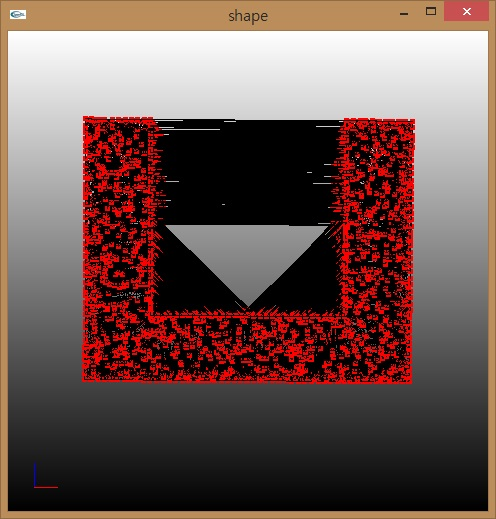
\includegraphics[height=4.0cm]{./figs/U_e.jpg}}
\subfigure[Vertices]{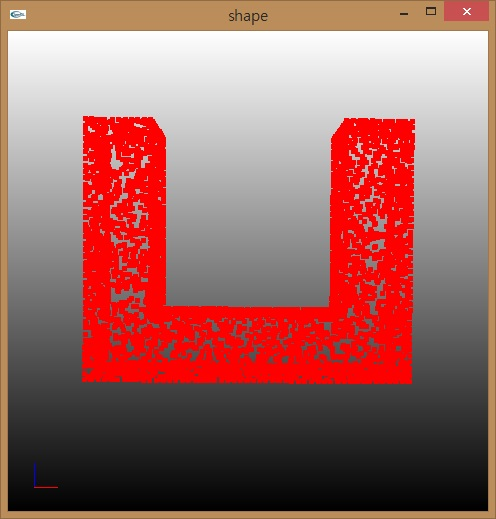
\includegraphics[height=4.0cm]{./figs/U_v.jpg}}
\subfigure[Tetrahedrons]{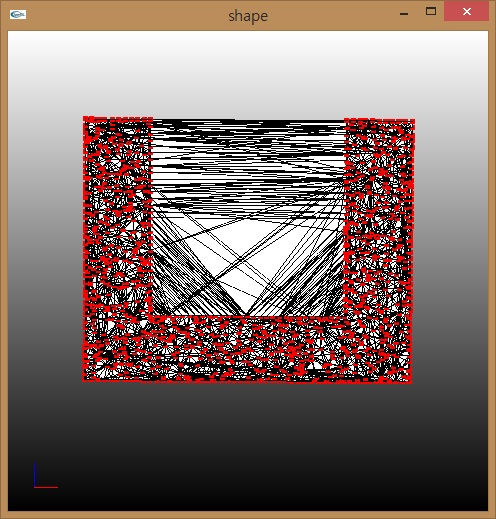
\includegraphics[height=4.0cm]{./figs/U_t.jpg}}
\caption{i.U}
\label{fig:U}
\end{figure}

\begin{figure}[!htb]
\centering
\subfigure[Faces and vertices]{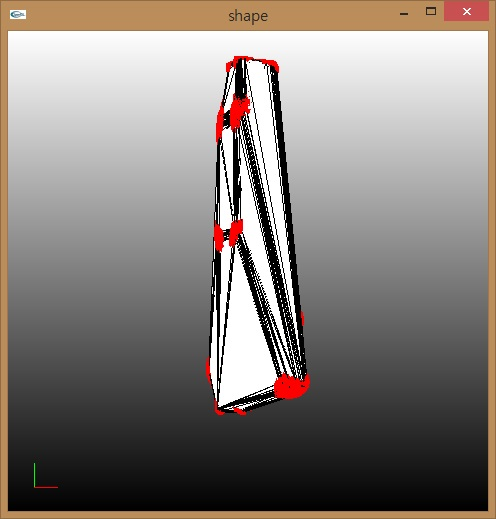
\includegraphics[height=4.0cm]{./figs/woman_f.jpg}}
\subfigure[Edges and vertices]{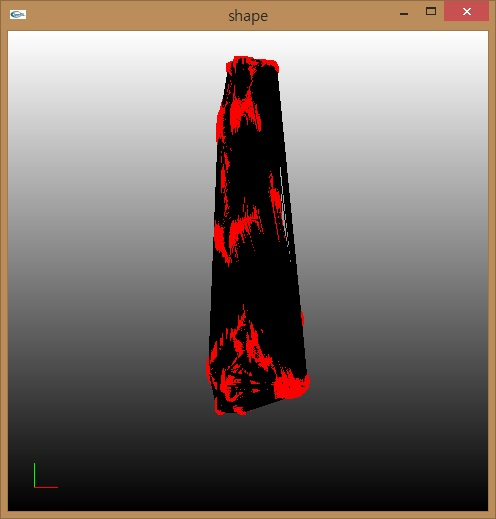
\includegraphics[height=4.0cm]{./figs/woman_e.jpg}}
\subfigure[Vertices]{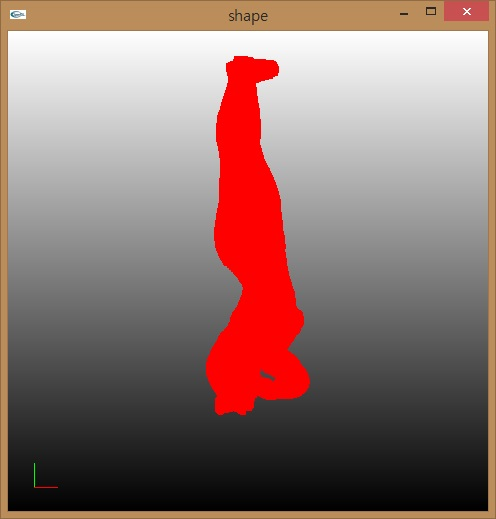
\includegraphics[height=4.0cm]{./figs/woman_v.jpg}}
\subfigure[Tetrahedrons]{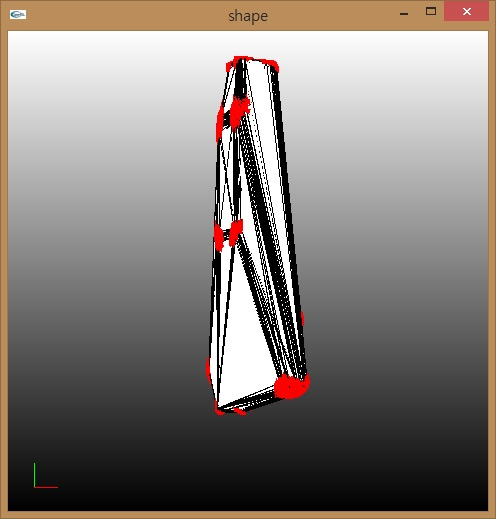
\includegraphics[height=4.0cm]{./figs/woman_t.jpg}}
\caption{i.woman}
\label{fig:woman}
\end{figure}

\begin{figure}[!htb]
\centering
\subfigure[Faces and vertices]{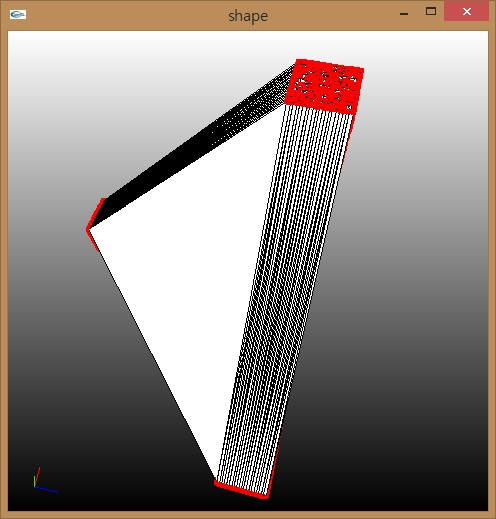
\includegraphics[height=4.0cm]{./figs/Y_f.jpg}}
\subfigure[Edges and vertices]{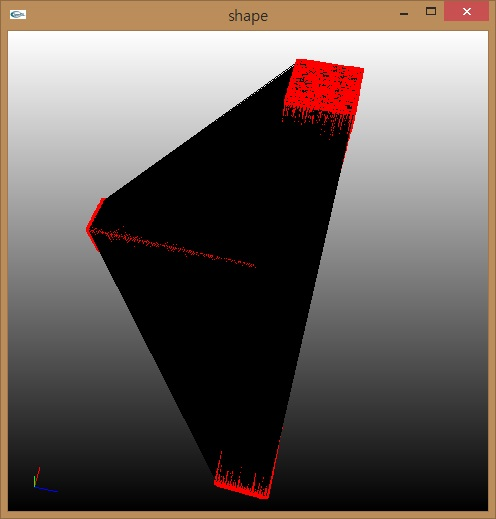
\includegraphics[height=4.0cm]{./figs/Y_e.jpg}}
\subfigure[Vertices]{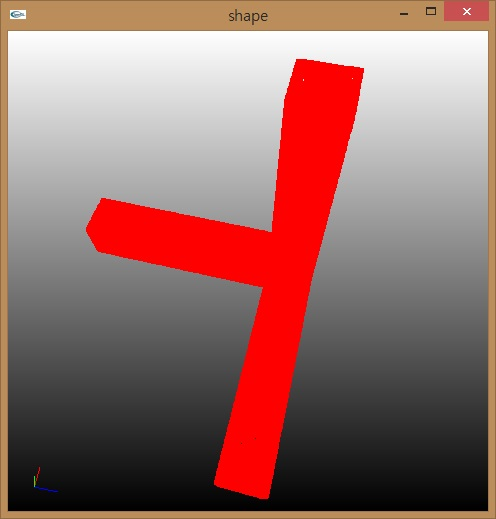
\includegraphics[height=4.0cm]{./figs/Y_v.jpg}}
\subfigure[Tetrahedrons]{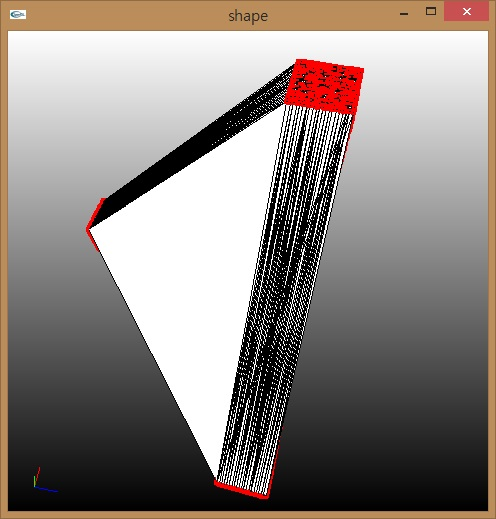
\includegraphics[height=4.0cm]{./figs/Y_t.jpg}}
\caption{i.Y}
\label{fig:Y}
\end{figure}

\section{Know bugs/limitations}

The program does not check duplication of edges. A edge exists as many as the adjacent faces in $edges$ since the program inserts all edges according to faces. Also $face$ in $tetras$, $edge$ in $faces$ and $adjface$ in $edges$ are not implemented but they does not influence on the results. The results are not close to the original model. It may approximate concave shapes to convex shapes such as ears of the bunny (Fig.~\ref{fig:bunny}). However, it shows perfect matching for convex models as illustrated in Fig.~\ref{fig:cube} and~\ref{fig:ellipsoid}. The program requires more method such as alpha shape to remove extra convex areas.

%\bibliographystyle{plain}
%\bibliography{report}

\end{document}


